%%%%%%%%%%%%%%%%%%%%%%%%%%%%%%%%%%%%%%%%%%%%%%%%%%%%%%%%%%%%%%%%%%%%%%%%%%%%%%%%
%%                          uAlberta Thesis Template                          %%
%%                                     by                                     %%
%%                               Daniel Aldrich                               %%
%%                               Version: 2.0.0                               %%
%%%%%%%%%%%%%%%%%%%%%%%%%%%%%%%%%%%%%%%%%%%%%%%%%%%%%%%%%%%%%%%%%%%%%%%%%%%%%%%%
%                                                                              %
%       Copyright (c) 2024 Daniel Aldrich                                      %
%                                                                              %
%       Permission is hereby granted, free of charge, to any person            %
%       obtaining a copy of this software and associated documentation         %
%       files (the "Software"), to deal in the Software without                %
%       restriction, including without limitation the rights to use,           %
%       copy, modify, merge, publish, distribute, sublicense, and/or           %
%       sell copies of the Software, and to permit persons to whom the         %
%       Software is furnished to do so, subject to the following               %
%       conditions:                                                            %
%                                                                              %
%       The above copyright notice and this permission notice shall be         %
%       included in all copies or substantial portions of the Software.        %
%                                                                              %
%       THE SOFTWARE IS PROVIDED "AS IS", WITHOUT WARRANTY OF ANY KIND,        %
%       EXPRESS OR IMPLIED, INCLUDING BUT NOT LIMITED TO THE WARRANTIES        %
%       OF MERCHANTABILITY, FITNESS FOR A PARTICULAR PURPOSE AND               %
%       NONINFRINGEMENT. IN NO EVENT SHALL THE AUTHORS OR COPYRIGHT            %
%       HOLDERS BE LIABLE FOR ANY CLAIM, DAMAGES OR OTHER LIABILITY,           %
%       WHETHER IN AN ACTION OF CONTRACT, TORT OR OTHERWISE, ARISING           %
%       FROM, OUT OF OR IN CONNECTION WITH THE SOFTWARE OR THE USE OR          %
%       OTHER DEALINGS IN THE SOFTWARE.                                        %
%                                                                              %
%%%%%%%%%%%%%%%%%%%%%%%%%%%%%%%%%%%%%%%%%%%%%%%%%%%%%%%%%%%%%%%%%%%%%%%%%%%%%%%%

%LIST OF AVAILABLE THEOREM ENVIRONMENTS
	% For the full list of available theorems OR to add your own theorems see
	%   the `includeTheroems.tex' file located in the 00_LaTeX_Files Folder.
	%
	% To use:
	% \begin{<theorem name>}
	%     <YOUR TEXT HERE>
	% \end{<theorem name>}

% Write command to allow the nomenclature to be generated properly.
\immediate\write18{makeindex \jobname.nlo -s nomencl.ist -o \jobname.nls}


\documentclass[
	pdfa,
	oneside,
	chapterbib,
	saychapapp,
	fancyheaders]{ualberta}
	% OPTIONS FOR ualberta.cls:
	% chapterbib - Automatically prints references at the end of each chapter.
	%
	% pdfa - To convert the PDF to PDF/A format (REQUIRED for GPS Submission)
	%
	% oneside - Standard for submitting to GPS.
	%
	% twoside - If you want to print your thesis double sided like a novel.
	%            Note: GPS requires the submission to be one sided. Please use
	%            the option `oneside' for submission to GPS.
	%
	% saychapapp - If you want your thesis to say Chapter # and Appendix @ in
	%               the ToC instead of just having the # or @.
	%               (GPS is inconsistent on if this is truly a Requirement.)
	%
	% fancyheader - If you want your thesis to have chapter headers rather than
	%               just a page number at the bottom.

% Option to change the Level of subheading included in the Table of Contents
%  This should be set at 2, 3, or 4 (As per GPS)
	\settoclevel{3}

%%%%%%%%%%%%%%%%%%%%%%%%%%%%%%%%%%%%%%%%%%%%%%%%%%%%%%%%%%%%%%%%%%%%%%%%%%%%%%%%
%                                FILE LOCATIONS                                %
%%%%%%%%%%%%%%%%%%%%%%%%%%%%%%%%%%%%%%%%%%%%%%%%%%%%%%%%%%%%%%%%%%%%%%%%%%%%%%%%
% The following Commands Can be set to change the lookup locations for files.
% LaTeX FILES LOCATION
	% .  - This folder
	% .. - Up one Folder
	\addlatexfiles{./00_LaTeX_Files/}
	\insertlatexfile{includePackages} % LOAD ALL PACKAGES TO BE INCLUDED

% PREFATORY LOCATION
	% .  - This folder
	% .. - Up one Folder
	\addprefatory{./01_Prefatory/}

% CHAPTER LOCATION
	% .  - This folder
	% .. - Up one Folder
	\addchapters{./02_Chapters/}

% BIBLIOGRAPHY LOCATION
	% NOTE: if you add bibliography entries after a compilation, you might notice
	%  references marked `[0]' to fix this just delete the auxiliary files.
	%  (*.aux, *.bbl, ... etc)
	%
	% .  - This folder
	% .. - Up one Folder
	\addbibresource{./03_References/References.bib}

% APPENDICES LOCATION
	% .  - This folder
	% .. - Up one Folder
	\addappendices{./04_Appendices/}

% MEDIA LOCATIONS
	% .  - This folder
	% .. - Up one Folder
	\addmedia{./99_Inclusions/}
	\addimages{Images/}
	\addtables{Tables/}
	\addcode{Code/}
	\adddata{Data/}
	\addpdf{PDFs/}

%%%%%%%%%%%%%%%%%%%%%%%%%%%%%%%%%%%%%%%%%%%%%%%%%%%%%%%%%%%%%%%%%%%%%%%%%%%%%%%%
%                         ADD ADDITIONAL RESOURCES                             %
%%%%%%%%%%%%%%%%%%%%%%%%%%%%%%%%%%%%%%%%%%%%%%%%%%%%%%%%%%%%%%%%%%%%%%%%%%%%%%%%
	\insertlatexfile{includeTheorems}
	\insertlatexfile{includeMacros}
	\insertlatexfile{listingCodeFormatting}

%%%%%%%%%%%%%%%%%%%%%%%%%%%%%%%%%%%%%%%%%%%%%%%%%%%%%%%%%%%%%%%%%%%%%%%%%%%%%%%%
%                  TITLE PAGE AND FRONTMATTER INFORMATION                      %
%%%%%%%%%%%%%%%%%%%%%%%%%%%%%%%%%%%%%%%%%%%%%%%%%%%%%%%%%%%%%%%%%%%%%%%%%%%%%%%%
% TITLE PAGE INFO
	\title{Thesis Title}                         % Title of your Thesis
	\author{First Middle Last}                   % Your Full Name
	\degree{\insertlatexfile{selectDegree}}      % Uncomment Degree in file
	\specialization{}                            % Leave blank if none
	\deptfac{\insertlatexfile{selectDepartment}} % Uncomment Department in file
	\convocationdate{\the\year}                  % Convocation Year

% ABSTRACT
	\insertprefatory{Abstract}

% PREFACE
	\insertprefatory{Preface}

% DEDICATION OR QUOTE
	\insertprefatory{Quotes_Dedications}

% ACKNOWLEDGEMENTS
	\insertprefatory{Acknowledgements}


%%%%%%%%%%%%%%%%%%%%%%%%%%%%%%%%%%%%%%%%%%%%%%%%%%%%%%%%%%%%%%%%%%%%%%%%%%%%%%%%
%                  NOMENCLATURE, GLOSSARY, ACRONYMS, ETC                       %
%%%%%%%%%%%%%%%%%%%%%%%%%%%%%%%%%%%%%%%%%%%%%%%%%%%%%%%%%%%%%%%%%%%%%%%%%%%%%%%%

% NOMENCLATURE
	\insertprefatory{Nomenclature}

% ACRONYMS
	\insertprefatory{Acronyms}

% GLOSSARY
	\insertprefatory{Glossary}


%%%%%%%%%%%%%%%%%%%%%%%%%%%%%%%%%%%%%%%%%%%%%%%%%%%%%%%%%%%%%%%%%%%%%%%%%%%%%%%%
%                              BEGIN DOCUMENT                                  %
%%%%%%%%%%%%%%%%%%%%%%%%%%%%%%%%%%%%%%%%%%%%%%%%%%%%%%%%%%%%%%%%%%%%%%%%%%%%%%%%
\begin{document}

	\maketitle                   % Creates the Title Page
	\makeabstract                % Creates the Abstract Page
	\makepreface                 % Creates the Preface Page
	% Quote and Dedication (Only Uncomment one)
		%\makequote                  % Creates the Quote Page
		%\makededication             % Creates the Dedication Page
		\makededicationandquote      % Creates the Quote/Dedication Page
	\acknowledgements            % Creates the Acknowledgements Page

% SET ToC...etc SPACING
	%\singlespacing              % 1.00x Spacing
	\onehalfspacing              % 1.50x Spacing
	%\doublespacing              % 1.75x Spacing
	%\truedoublespacing          % 2.00x Spacing
	%\triplespacing              % 3.00x Spacing
	%\baselineskip #.##em        % #.##x Spacing

% ALL LISTS/TABLES OF ________
% Everything below should Automatically be included if it has content and
%  excluded if it does not. There is no need to comment any line here. If you
%  would like a different order however feel free to move items to new lines.
	\tableofcontents             % Creates the Table of Contents
	\listoftables                % Creates the List of Tables
	\listoffigures               % Creates the List of Figures
	\listofplates                % Creates the List of Plates (photographs)
	\listofsymbols               % Creates the List of Symbols (Nomenclature)
	\abbreviations               % Creates the List of Acronyms (Abbreviations)
	\glsaddall                   % Required for List of Acronyms and Glossary
	\generateglossary            % Creates the Glossary of Terms


%%%%%%%%%%%%%%%%%%%%%%%%%%%%%%%%%%%%%%%%%%%%%%%%%%%%%%%%%%%%%%%%%%%%%%%%%%%%%%%%
%                           ADD YOUR CONTENT HERE                              %
%%%%%%%%%%%%%%%%%%%%%%%%%%%%%%%%%%%%%%%%%%%%%%%%%%%%%%%%%%%%%%%%%%%%%%%%%%%%%%%%
	\bodyoftext % Switches the style of the document to that of the body

% SET DOCUMENT SPACING
	%\onehalfspacing       % 1.50x Spacing **Minimum Spacing for the THESIS BODY
	%\doublespacing        % 1.75x Spacing
	\truedoublespacing     % 2.00x Spacing **Required for the ABSTRACT
	%\triplespacing        % 3.00x Spacing
	%\baselineskip #.##em  % #.##x Spacing

% To insert chapters from a separate tex file use the following commands
% \insertchapter automatically looks in the Chapters folder and also
%   appends the file extension (i.e. do NOT include the '.tex')
%
% \input is the standard way of including a separate tex file
% \chapter{Example Chapter}\label{ch:Example}
  This chapter aims to provide examples how how to structure and create specific components in your thesis document. The very first one is showing a citation, like the one at the end of this sentence \cite{TEST}. The second shows how to create more than one citation and how they are grouped \cite{testone,cite2,cite3,cite4,cite5}.
This sentence shows how a gap in the citations is handled \cite{testone,cite2,cite3,cite5}. 
  \section{Tables}
  
  % L - Left Aligned (Equal Spacing)
  % C - Center Aligned (Equal Spacing)
  % R - Right Aligned (Equal Spacing)
  % l - Left Aligned (Fit to Contents)
  % c - Center Aligned (Fit to Contents)
  % r - Right Aligned (Fit to Contents)
  
  \begin{table}[!htb]
    \caption{This is a basic table}
    \centering
    \begin{tabularx}{0.75\textwidth}{LCR} 
      % Equally spaced cells that are left, center, and reight aligned. 
      % The entire table will be 75% the width of the text.
      \hline
      \textbf{Left Aligned Title} & \textbf{Centered Title} & \textbf{Right Aligned Title} \\\hline
      This is left aligned & This is centered & This is right aligned \\
      This is left aligned & This is centered & This is right aligned \\
      This is left aligned & This is centered & This is right aligned \\
      This is left aligned & This is centered & This is right aligned \\\hline
    \end{tabularx}
    \label{tab:basicTable}
  \end{table}
  
  \begin{table}[!htb]
    \caption{This is a complex table.}
    \centering
    \begin{tabularx}{\textwidth}{lCR}
      % Left most cell is fitted to the content.
      % The center and right columns are equally spaced cells that are center, and reight aligned. 
      % The entire table will be 75% the width of the text.
      \hline
      \multirow{2}{*}{\textbf{This is two row\quad}} & \multicolumn{2}{c}{\textbf{This is two columns}}\\\cline{2-3} % \cline draws a partial line across cells #-#
       & \textbf{Centered Title} & \textbf{Right Aligned Title} \\\hline
      \multirow{2}{*}{This is two row} & This is centered & This is right aligned \\
       & This is centered & This is right aligned \\\cline{1-1}
      \multirow{2}{*}{This is two row} & This is centered & This is right aligned \\
       & This is centered & This is right aligned \\\hline
    \end{tabularx}
    \label{tab:complexTable}
  \end{table}
  
  
  \section{Figures}
  This section will provide examples of how to create figures, and different types of multi/sub-figures. Additionally, if you have many figures in a section and they are bleeding too much into the following sections a \textbackslash{}clearpage command can be issued before the next section. However, note that this will force the next section to begin on a new page. Note that the first ``figure'' is actually a plate; a plate is the proper title associated with a photograph, using the environment `plate' instead of figure and command listofplates will generate everything for you.
  \begin{plate}[!htb]
    \centering
    \includegraphics[width=0.7\textwidth]{example-image}
    \caption{This is an example of a single image plate.}
    \label{fig:singleImage}
  \end{plate}
  
  \begin{figure}[!htb]
    \centering
    \begin{subfigure}{0.45\textwidth}
      \includegraphics[width=\textwidth]{example-image}
      \caption{} % Leave blank for just letter
      \label{fig:doubleImage:a}
    \end{subfigure}
    ~
    \begin{subfigure}{0.45\textwidth}
      \includegraphics[width=\textwidth]{example-image}
      \caption{} % Leave blank for just letter
      \label{fig:doubleImage:b}
    \end{subfigure}
    \caption{This is an example of a double image figure.}
    \label{fig:doubleImage}
  \end{figure}
  
  \begin{figure}[!htb]
    \centering
    \hspace*{\fill}% Adds space to left of top image (prevents two images from going to top)
    \begin{subfigure}{0.45\textwidth}
      \includegraphics[width=\textwidth]{example-image}
      \caption{} % Leave blank for just letter
      \label{fig:tripleImage:a}
    \end{subfigure}
    \hspace*{\fill} % Adds space to right of top image (prevents two images from going to top)
    \par\vspace{1em}% Adds space between upper and lower images
    \begin{subfigure}{0.45\textwidth}
      \includegraphics[width=\textwidth]{example-image}
      \caption{} % Leave blank for just letter
      \label{fig:tripleImage:b}
    \end{subfigure}
    ~ % Adds space between the two lower figures
    \begin{subfigure}{0.45\textwidth}
      \includegraphics[width=\textwidth]{example-image}
      \caption{} % Leave blank for just letter
      \label{fig:tripleImage:c}
    \end{subfigure}
    \caption{This is an example of a triple image figure.}
    \label{fig:tripleImage}
  \end{figure}
  
  \begin{figure}[!htb]
    \centering
    \hspace*{\fill}% Adds space to left of top image (prevents two images from going to top)
    \begin{subfigure}{0.90\textwidth+1em} % 0.9 = 0.45 + 0.45, and 1em is the width of ~
      \includegraphics[width=\textwidth]{example-image}
      \caption{} % Leave blank for just letter
      \label{fig:tripleImage:a}
    \end{subfigure}
    \hspace*{\fill} % Adds space to right of top image (prevents two images from going to top)
    \par\vspace{1em}% Adds space between upper and lower images
    \begin{subfigure}{0.45\textwidth}
      \includegraphics[width=\textwidth]{example-image}
      \caption{} % Leave blank for just letter
      \label{fig:tripleImage:b}
    \end{subfigure}
    ~ % Adds space between the two lower figures
    \begin{subfigure}{0.45\textwidth}
      \includegraphics[width=\textwidth]{example-image}
      \caption{} % Leave blank for just letter
      \label{fig:tripleImage:c}
    \end{subfigure}
    \caption{This is a second example of a triple image figure.}
    \label{fig:tripleImage}
  \end{figure}
  
  \begin{figure}[!htb]
    \centering
    \begin{subfigure}{0.45\textwidth}
      \includegraphics[width=\textwidth]{example-image}
      \caption{} % Leave blank for just letter
      \label{fig:quadImage:a}
    \end{subfigure}
    ~ % Adds space between the two top figures
    \begin{subfigure}{0.45\textwidth}
      \includegraphics[width=\textwidth]{example-image}
      \caption{} % Leave blank for just letter
      \label{fig:quadImage:b}
    \end{subfigure}
    \par\vspace{1em} % Adds space between upper and lower images
    \begin{subfigure}{0.45\textwidth}
      \includegraphics[width=\textwidth]{example-image}
      \caption{} % Leave blank for just letter
      \label{fig:quadImage:c}
    \end{subfigure}
    ~ % Adds space between the two lower figures
    \begin{subfigure}{0.45\textwidth}
      \includegraphics[width=\textwidth]{example-image}
      \caption{} % Leave blank for just letter
      \label{fig:quadImage:d}
    \end{subfigure}
    \caption{This is an example of a quad image figure.}
    \label{fig:quadImage}
  \end{figure}
  
  \clearpage % forces the remaining images (floats to be placed)
  \section{Equations}
  The following equation has no referencing number:
  \nonumeq{E = & m\ c^2}
  
  \Cref{eq:quickEq} has a reference to it though. Or for more control the source for \Cref{eq:quickEq} can be written out fully as it was for \Cref{eq:quickEq2}.
  
  \numeq{pi = & 3.1415...}{eq:quickEq} % shorthand for the following way of writing equations.
  \begin{align}\label{eq:quickEq2}
    e = & 2.7183...
  \end{align}
  
  If you have multiple equations that you want arranged very neatly, use the align environment and you can assign individual equations numbers as shown in \Cref{eq:multiref:a,eq:multiref:b,eq:multiref:c}.
  \begin{align}%Note: Alignment happens at the "=" character
    \label{eq:multiref:a} Equation1 = & 1 + 1\\
    \label{eq:multiref:b} Equation2 = & 2 + 2\\
    \label{eq:multiref:c} Equation3 = & 3 + 3
  \end{align}
  
  
  
  \printreferences % Add a Reference Section to the end of the Chapter.

	\insertchapter{01_Introduction}
	\insertchapter{02_Getting_Started}
	\insertchapter{03_Document_Structure}
	\insertchapter{04_Figures_Tables}
	\insertchapter{05_Plots_And_Graphs}
	\insertchapter{06_Mathematical_Equations}
	\insertchapter{07_Citations_And_References}

% How to use the Recommended Softwares
	\insertchapter{08_JabRef}

	\insertchapter{XX_Submitting_Your_Thesis}

	%\insertchapter{09_TeXstudio}

	%\insertchapter{10_dia}

	%\insertchapter{11_}

	%\insertchapter{12_}

	%\insertchapter{13_}

	%\insertchapter{14_}

	%\insertchapter{02_Example_Chapter}
	%\insertchapter{0X_Background}
	%\insertchapter{0X_Paper_1}
	%\insertchapter{0X_Paper_2}
	%\insertchapter{0X_Conclusions_Recommendations_and_Future_Work}


%%%%%%%%%%%%%%%%%%%%%%%%%%%%%%%%%%%%%%%%%%%%%%%%%%%%%%%%%%%%%%%%%%%%%%%%%%%%%%%%
%                                 BIBLIOGRAPHY                                 %
%%%%%%%%%%%%%%%%%%%%%%%%%%%%%%%%%%%%%%%%%%%%%%%%%%%%%%%%%%%%%%%%%%%%%%%%%%%%%%%%

% Uncomment the \nocite{*} if you want to include works read, but not cited
%   within the body of your work.
	% \nocite{*}
	\printbibliography[heading=bibintoc]


%%%%%%%%%%%%%%%%%%%%%%%%%%%%%%%%%%%%%%%%%%%%%%%%%%%%%%%%%%%%%%%%%%%%%%%%%%%%%%%%
%                                  APPENDICES                                  %
%%%%%%%%%%%%%%%%%%%%%%%%%%%%%%%%%%%%%%%%%%%%%%%%%%%%%%%%%%%%%%%%%%%%%%%%%%%%%%%%
\appendix
% SET APPENDIX SPACING
	%\onehalfspacing              % 1.50x Spacing
	%\doublespacing               % 1.75x Spacing
	\truedoublespacing            % 2.00x Spacing
	%\triplespacing               % 3.00x Spacing
	%\baselineskip #.##em         % #.##x Spacing

% To insert appendices from a separate tex file use the following commands
% \insertappendix automatically looks in the Appendices folder and also
%   appends the file extension (i.e. do NOT include the '.tex'
%
% \input is the standard way of including a separate tex file
% \chapter{Inserting PDFs}\label{sec:motorSpecs}
% NOTE: the PDFs are inserted at 85% their full size to ensure that they don't overlap any FGSR page formatting required for the headers and footers.
  \section{how to insert a portrait PDF}
    
\includepdf[landscape=false,pages=-,pagecommand={},scale=0.85]{./Appendices/examplePDF}
  \section{How to insert a landscape PDF}
    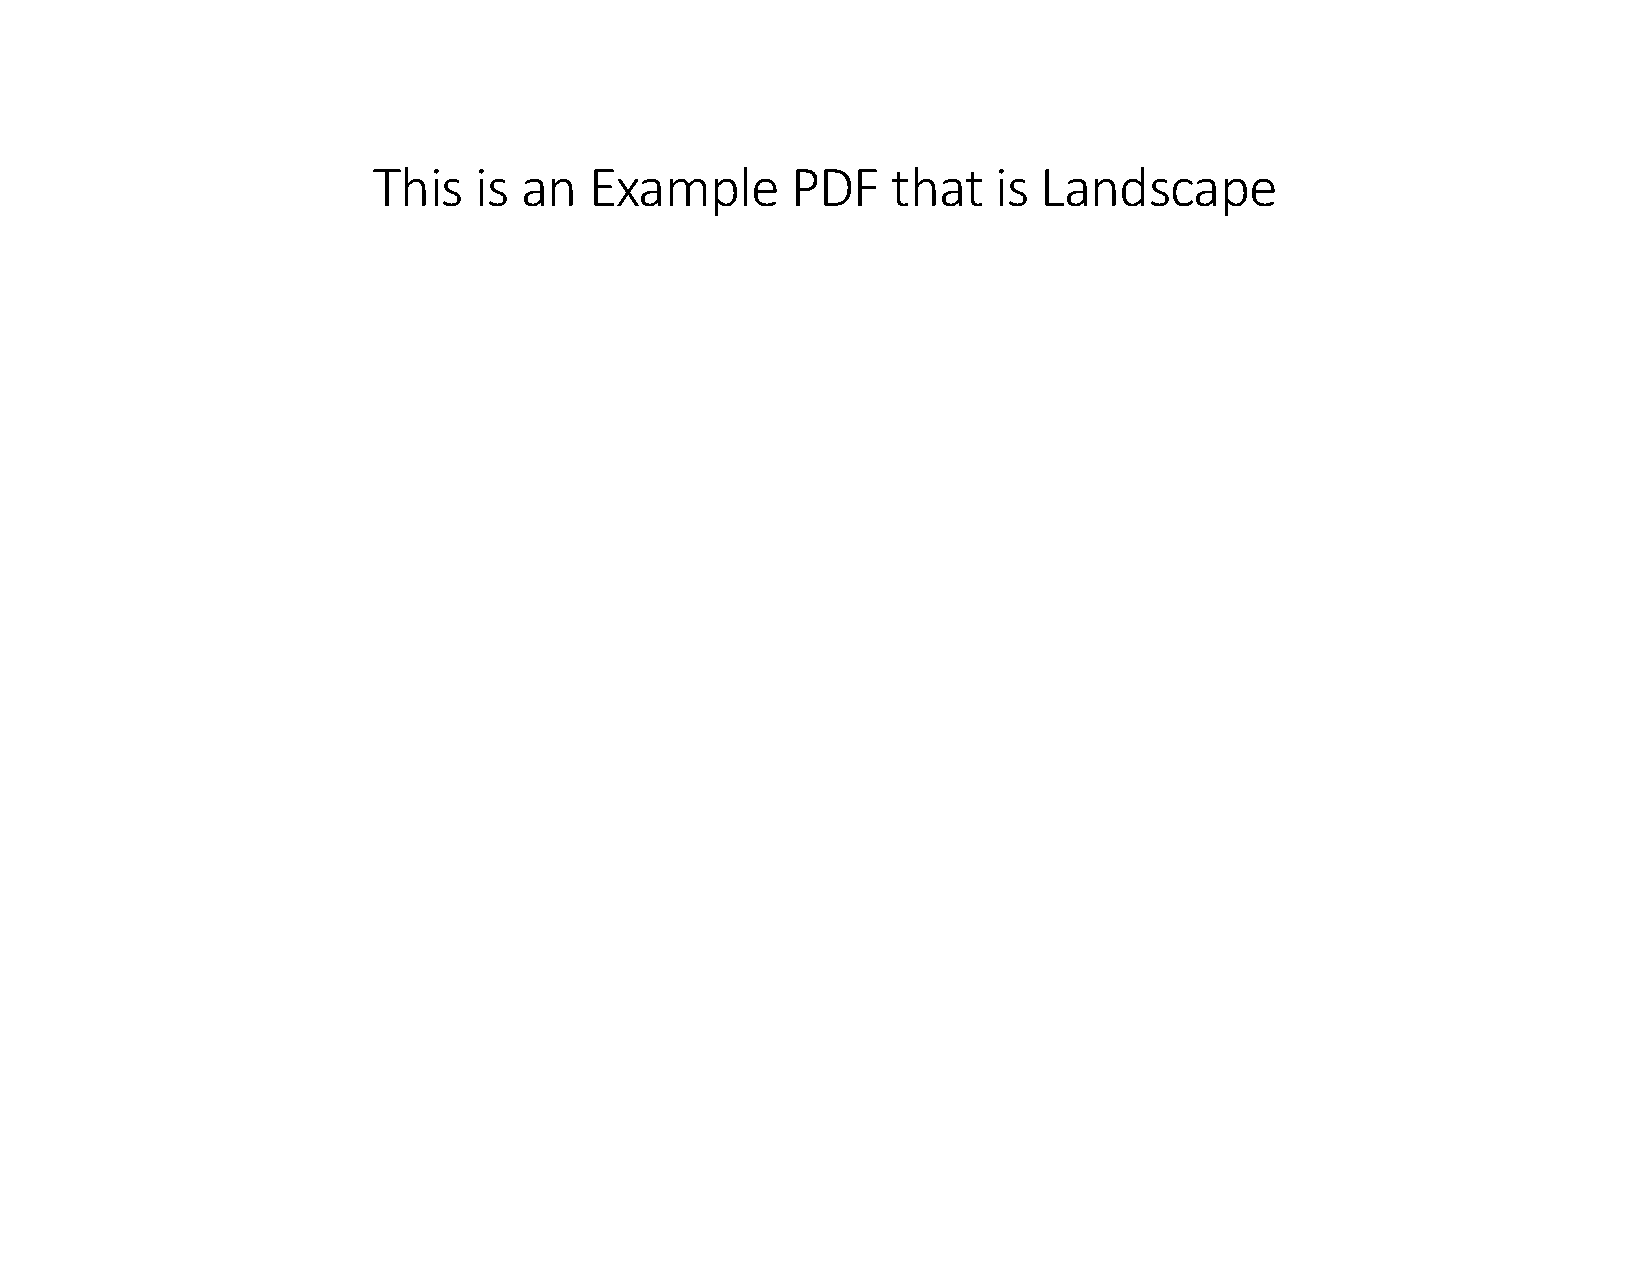
\includepdf[landscape=true,pages=-,pagecommand={},scale=0.85]{./Appendices/landscapePDF}

	\insertappendix{0A_Additional_Figures}

	\insertappendix{0B_Additional_Tables}

	\insertappendix{0C_Code_Listings}

	\insertappendix{0D_Including_PDFs}

	\insertappendix{0X_Math_Lettering}

\end{document}
